\section{Finding Elusive Hardware Monitors}
\label{sec:elusive_hardware_monitors}
\begin{figure}[hbt!]
\centering
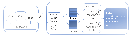
\includegraphics[width=\columnwidth]{\chapterdirectory/figure/micro_bench/expose_monitor_general_approach.pdf}
\caption{%
Trace collection process (extracted from \cite{palomo_et_al:LIPIcs:2020:12378})
}
\label{fig:micro_bench:expose_monitors}
\end{figure}

\cite{palomo_et_al:LIPIcs:2020:12378} presents a case study for the profiling of
architectures where performance monitors are not available. This is interesting,
because architecture profiling usually assumes that they are available. Having
a way to profile architectures without would extend the range of architectures
that can be considered for critical real-time contexts.

The architecture being studied in \cite{palomo_et_al:LIPIcs:2020:12378} is
system-on-chip with a dual-core processor.  While it does not have performance
monitors, it does have some hardware debugging features, which can be accessed
using a \textit{JTAG} port.

These hardware debugging features can snoop the messages passing through the
interconnect, as well as the instructions executed by each core (and their
program counter). In the approach proposed by
\cite{palomo_et_al:LIPIcs:2020:12378}, the platform is configured so that these
two sources of information are stored into circular buffers (within the chip).
The \textit{JTAG} connection is used to continuously copy these buffers into an
external analysis platform (see Figure~\ref{fig:micro_bench:expose_monitors}).
The speed at which these buffers are filled is higher than that of the
\textit{JTAG} connection, meaning that information would be lost if the programs
were running normally. Thus, the \textit{GRMON} script takes control of the
execution once the section of the programs under analysis is reached, and
proceeds to running the applications in a \textit{step-by-step} manner, which
ensures no information is lost.

Once this event capture is completed, the post-processing steps begin, starting
with a clean-up phase (\textit{Trace Merging}), which clears out redundant data.
Then comes the \textit{Event Counting} phase, which matches instructions to bus
events in order to recognize patterns that fit known events. For example, data
cache load misses are identified by seeing a load instruction be performed by
a core one cycle \textit{after} seeing the matching query go through the
interconnect.

Thus, instead of relying on performance counters, it is possible to obtain an
accurate description of the behavior of the platform through capture and
analysis of execution traces. Such strategies extend the range of platforms upon
which profiling is possible, including for the purpose of identifying cache
coherence using the process described in
Chapter~\ref{cha:identifying_cache_coherence}.
